\documentclass[tikz]{standalone}

\usepackage{mathtools}

\newcommand{\Acal}{\boldsymbol{\mathcal{A}}}
\newcommand{\Ccal}{\boldsymbol{\mathcal{C}}}
\newcommand{\add}{{\boldsymbol{\oplus}}}

\begin{document}
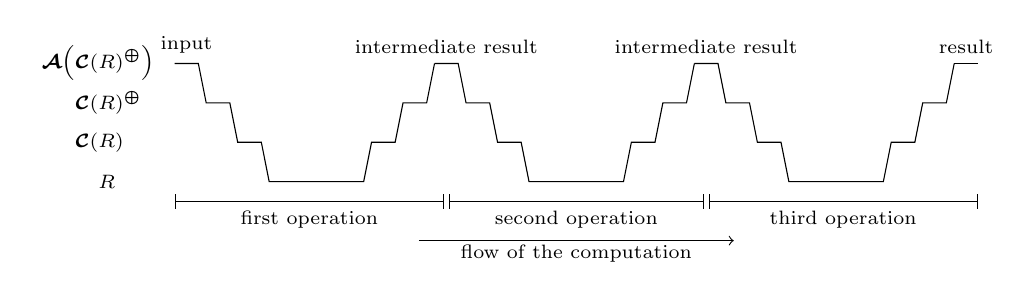
\begin{tikzpicture}
	\def\yfactor{0.5}
	\node [align=right, text width=1.5cm] at (-1,0*\yfactor) {\scriptsize{$\Acal\Big(\Ccal(R)^\add\Big)$}};
	\node [align=right, text width=1.5cm] at (-1,-1*\yfactor) {\scriptsize{$\Ccal(R)^\add\hphantom{\Big)}$}};
\node [align=right, text width=1.5cm] at (-1,-2*\yfactor) {\scriptsize{$\Ccal(R)\hphantom{^\add\Big)}$}};
	\node [align=right, text width=1.5cm] at (-1,-3*\yfactor) {\scriptsize{$R\hphantom{)^\add\Big)}$}};
	\def\x{0}
	\draw (\x+0,0*\yfactor) -- node[above] {\scriptsize{input}} (\x+0.3,0*\yfactor) -- (\x+0.4,-1*\yfactor) -- (\x+0.7,-1*\yfactor) -- (\x+0.8,-2*\yfactor) -- (\x+1.1,-2*\yfactor) -- (\x+1.2,-3*\yfactor) -- (\x+2.4,-3*\yfactor) -- (\x+2.5,-2*\yfactor) -- (\x+2.8,-2*\yfactor) -- (\x+2.9,-1*\yfactor) -- (\x+3.2,-1*\yfactor) -- (\x+3.3,0*\yfactor);
	\def\x{3.3}
	\draw (\x+0,0*\yfactor) -- node[above] {\scriptsize{intermediate result}} (\x+0.3,0*\yfactor) -- (\x+0.4,-1*\yfactor) -- (\x+0.7,-1*\yfactor) -- (\x+0.8,-2*\yfactor) -- (\x+1.1,-2*\yfactor) -- (\x+1.2,-3*\yfactor) -- (\x+2.4,-3*\yfactor) -- (\x+2.5,-2*\yfactor) -- (\x+2.8,-2*\yfactor) -- (\x+2.9,-1*\yfactor) -- (\x+3.2,-1*\yfactor) -- (\x+3.3,0*\yfactor);
	\def\x{6.6}
	\draw (\x+0,0*\yfactor) -- node[above] {\scriptsize{intermediate result}} (\x+0.3,0*\yfactor) -- (\x+0.4,-1*\yfactor) -- (\x+0.7,-1*\yfactor) -- (\x+0.8,-2*\yfactor) -- (\x+1.1,-2*\yfactor) -- (\x+1.2,-3*\yfactor) -- (\x+2.4,-3*\yfactor) -- (\x+2.5,-2*\yfactor) -- (\x+2.8,-2*\yfactor) -- (\x+2.9,-1*\yfactor) -- (\x+3.2,-1*\yfactor) -- (\x+3.3,0*\yfactor);
	\draw (9.9,0*\yfactor) -- node[above] {\scriptsize{result}} (10.2,0*\yfactor);

	\draw [Bar-Bar] (0,-3.5*\yfactor) -- node[below] {\scriptsize{first operation}} (3.42,-3.5*\yfactor);
	\draw [Bar-Bar] (3.48,-3.5*\yfactor) -- node[below] {\scriptsize{second operation}} (6.72,-3.5*\yfactor);
	\draw [Bar-Bar] (6.78,-3.5*\yfactor) -- node[below] {\scriptsize{third operation}} (10.2,-3.5*\yfactor);

	\draw [->] (3.1,-4.5*\yfactor) -- node[below=-0.2em] {\scriptsize{flow of the computation}} (7.1,-4.5*\yfactor);
\end{tikzpicture}
\end{document}
